\section{Appendices}
In this appendix are included all the original black and white denoised images and its PSNR values. 

\begin{figure}[H]
  \centering
  \begin{tabular}{c c c c c}
      \begin{varwidth}{0.5\linewidth}
        \subfigure{\includegraphics[width=16mm]{Figures/results_mean/lena_nor_f.jpg}}\\
        \subfigure{\includegraphics[width=16mm]{Figures/results_mean/cameraman_nor_f.jpg}}\\
        \subfigure{\includegraphics[width=16mm]{Figures/results_mean/baboon_nor_f.jpg}}
      \end{varwidth}
      \begin{varwidth}{0.5\linewidth}
        \subfigure{\includegraphics[width=16mm]{Figures/results_mean/lena_ric_f.jpg}}\\
        \subfigure{\includegraphics[width=16mm]{Figures/results_mean/cameraman_ric_f.jpg}}\\
        \subfigure{\includegraphics[width=16mm]{Figures/results_mean/baboon_ric_f.jpg}}
      \end{varwidth}
      \begin{varwidth}{0.5\linewidth}
        \subfigure{\includegraphics[width=16mm]{Figures/results_mean/lena_uni_f.jpg}}\\
        \subfigure{\includegraphics[width=16mm]{Figures/results_mean/cameraman_uni_f.jpg}}\\
        \subfigure{\includegraphics[width=16mm]{Figures/results_mean/baboon_uni_f.jpg}}
      \end{varwidth}
      \begin{varwidth}{0.5\linewidth}
        \subfigure{\includegraphics[width=16mm]{Figures/results_mean/lena_sp_f.jpg}}\\
        \subfigure{\includegraphics[width=16mm]{Figures/results_mean/cameraman_sp_f.jpg}}\\
        \subfigure{\includegraphics[width=16mm]{Figures/results_mean/baboon_sp_f.jpg}}
      \end{varwidth}
      \begin{varwidth}{0.5\linewidth}
        \subfigure{\includegraphics[width=16mm]{Figures/results_mean/lena_spec.jpg}}\\
        \subfigure{\includegraphics[width=16mm]{Figures/results_mean/cameraman_spec.jpg}}\\
        \subfigure{\includegraphics[width=16mm]{Figures/results_mean/baboon_spec.jpg}}
      \end{varwidth}
  	\end{tabular}
  \caption{Denoised images with the mean filter. From left to right: removing Gaussian, Rician, uniform, salt and pepper and speckle noise, respectively.} 
  \label{fig:results_synthetic_mean}
\end{figure}

\begin{figure}[H]
  \centering
  \begin{tabular}{c c c c c}
      \begin{varwidth}{0.5\linewidth}
        \subfigure{\includegraphics[width=16mm]{Figures/results_median/lena_nor_f.jpg}}\\
        \subfigure{\includegraphics[width=16mm]{Figures/results_median/cameraman_nor_f.jpg}}\\
        \subfigure{\includegraphics[width=16mm]{Figures/results_median/baboon_nor_f.jpg}}
      \end{varwidth}
      \begin{varwidth}{0.5\linewidth}
        \subfigure{\includegraphics[width=16mm]{Figures/results_median/lena_ric_f.jpg}}\\
        \subfigure{\includegraphics[width=16mm]{Figures/results_median/cameraman_ric_f.jpg}}\\
        \subfigure{\includegraphics[width=16mm]{Figures/results_median/baboon_ric_f.jpg}}
      \end{varwidth}
      \begin{varwidth}{0.5\linewidth}
        \subfigure{\includegraphics[width=16mm]{Figures/results_median/lena_uni_f.jpg}}\\
        \subfigure{\includegraphics[width=16mm]{Figures/results_median/cameraman_uni_f.jpg}}\\
        \subfigure{\includegraphics[width=16mm]{Figures/results_median/baboon_uni_f.jpg}}
      \end{varwidth}
      \begin{varwidth}{0.5\linewidth}
        \subfigure{\includegraphics[width=16mm]{Figures/results_median/lena_sp_f.jpg}}\\
        \subfigure{\includegraphics[width=16mm]{Figures/results_median/cameraman_sp_f.jpg}}\\
        \subfigure{\includegraphics[width=16mm]{Figures/results_median/baboon_sp_f.jpg}}
      \end{varwidth}
      \begin{varwidth}{0.5\linewidth}
        \subfigure{\includegraphics[width=16mm]{Figures/results_median/lena_spec.jpg}}\\
        \subfigure{\includegraphics[width=16mm]{Figures/results_median/cameraman_spec.jpg}}\\
        \subfigure{\includegraphics[width=16mm]{Figures/results_median/baboon_spec.jpg}}
      \end{varwidth}
  	\end{tabular}
  \caption{Denoised images with the median filter. From left to right: removing Gaussian, Rician, uniform, salt and pepper and speckle noise, respectively.} 
  \label{fig:results_synthetic_median}
\end{figure}

\begin{figure}[H]
  \centering
  \begin{tabular}{c c c c c}
      \begin{varwidth}{0.5\linewidth}
        \subfigure{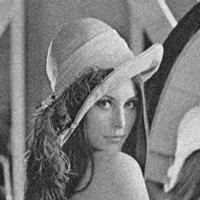
\includegraphics[width=16mm]{Figures/results_Lee/lena_nor-denoised.jpg}}\\
        \subfigure{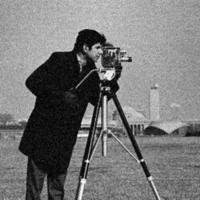
\includegraphics[width=16mm]{Figures/results_Lee/cameraman_nor-denoised.jpg}}\\
        \subfigure{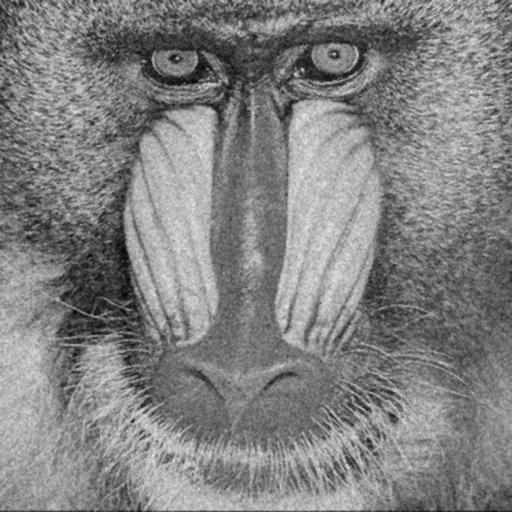
\includegraphics[width=16mm]{Figures/results_Lee/baboon_nor-denoised.jpg}}
      \end{varwidth}
      \begin{varwidth}{0.5\linewidth}
        \subfigure{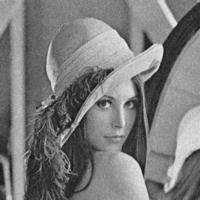
\includegraphics[width=16mm]{Figures/results_Lee/lena_ric-denoised.jpg}}\\
        \subfigure{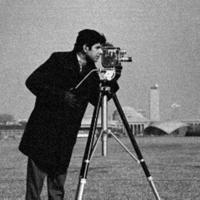
\includegraphics[width=16mm]{Figures/results_Lee/cameraman_ric-denoised.jpg}}\\
        \subfigure{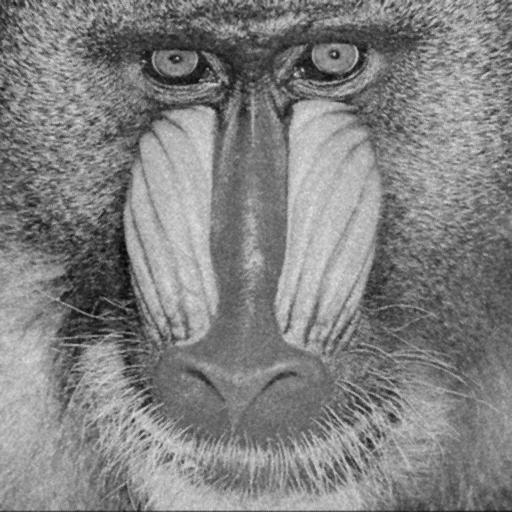
\includegraphics[width=16mm]{Figures/results_Lee/baboon_ric-denoised.jpg}}
      \end{varwidth}
      \begin{varwidth}{0.5\linewidth}
        \subfigure{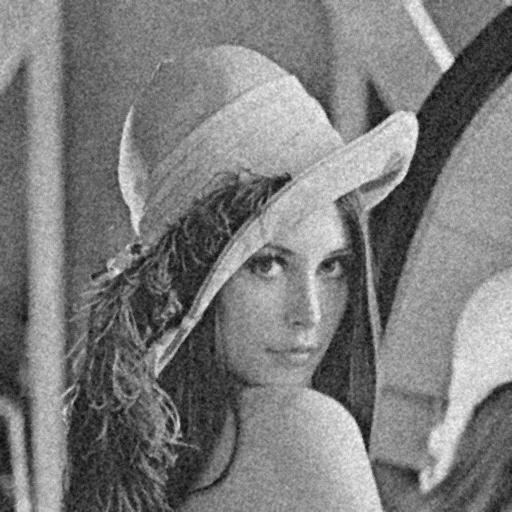
\includegraphics[width=16mm]{Figures/results_Lee/lena_uni-denoised.jpg}}\\
        \subfigure{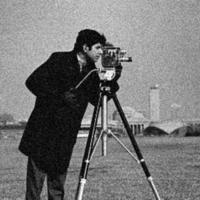
\includegraphics[width=16mm]{Figures/results_Lee/cameraman_uni-denoised.jpg}}\\
        \subfigure{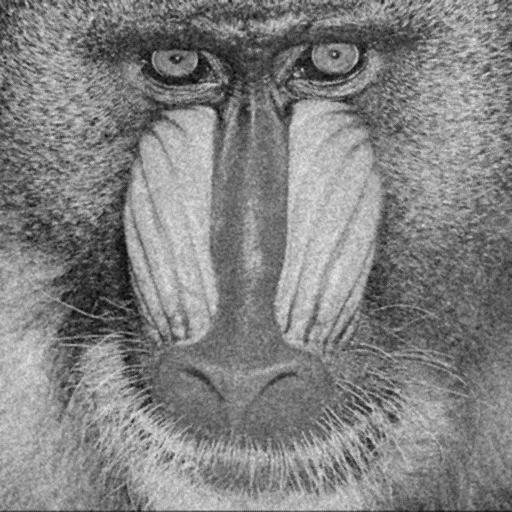
\includegraphics[width=16mm]{Figures/results_Lee/baboon_uni-denoised.jpg}}
      \end{varwidth}
      \begin{varwidth}{0.5\linewidth}
        \subfigure{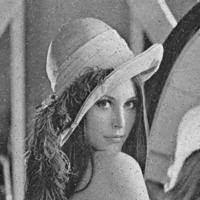
\includegraphics[width=16mm]{Figures/results_Lee/lena_sp-denoised.jpg}}\\
        \subfigure{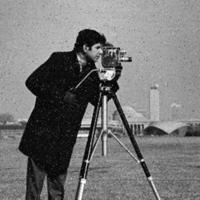
\includegraphics[width=16mm]{Figures/results_Lee/cameraman_sp-denoised.jpg}}\\
        \subfigure{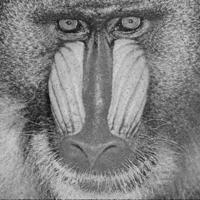
\includegraphics[width=16mm]{Figures/results_Lee/baboon_sp-denoised.jpg}}
      \end{varwidth}
      \begin{varwidth}{0.5\linewidth}
        \subfigure{\includegraphics[width=16mm]{Figures/results_Lee/lena_spec.jpg}}\\
        \subfigure{\includegraphics[width=16mm]{Figures/results_Lee/cameraman_spec.jpg}}\\
        \subfigure{\includegraphics[width=16mm]{Figures/results_Lee/baboon_spec.jpg}}
      \end{varwidth}
  	\end{tabular}
  \caption{Denoised images with the LS filter. From left to right: removing Gaussian, Rician, uniform, salt and pepper and speckle noise, respectively.} 
  \label{fig:results_synthetic_ls}
\end{figure}

\begin{figure}[H]
  \centering
  \begin{tabular}{c c c c c}
      \begin{varwidth}{0.5\linewidth}
        \subfigure{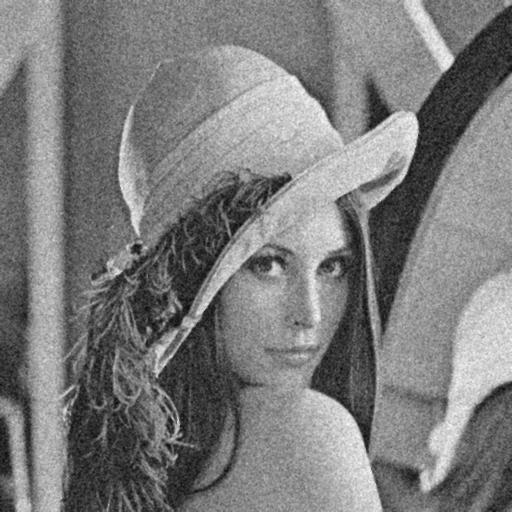
\includegraphics[width=16mm]{Figures/results_wavelet/lena_nor.jpg}}\\
        \subfigure{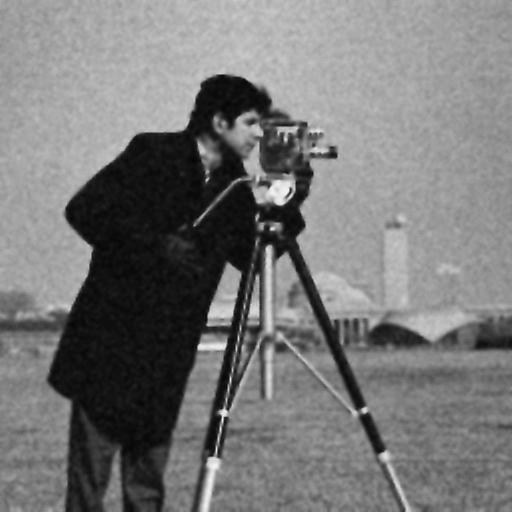
\includegraphics[width=16mm]{Figures/results_wavelet/cameraman_nor.jpg}}\\
        \subfigure{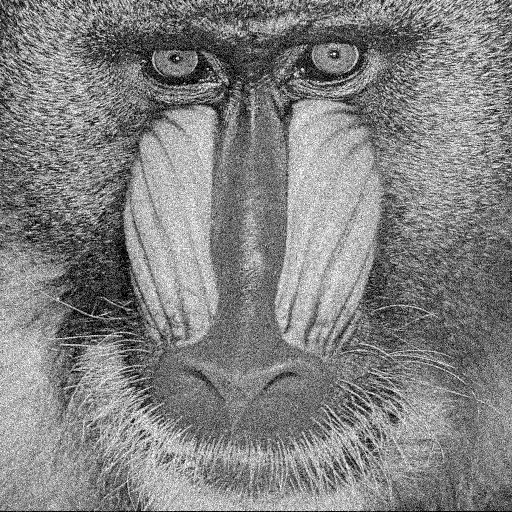
\includegraphics[width=16mm]{Figures/results_wavelet/baboon_nor.jpg}}
      \end{varwidth}
      \begin{varwidth}{0.5\linewidth}
        \subfigure{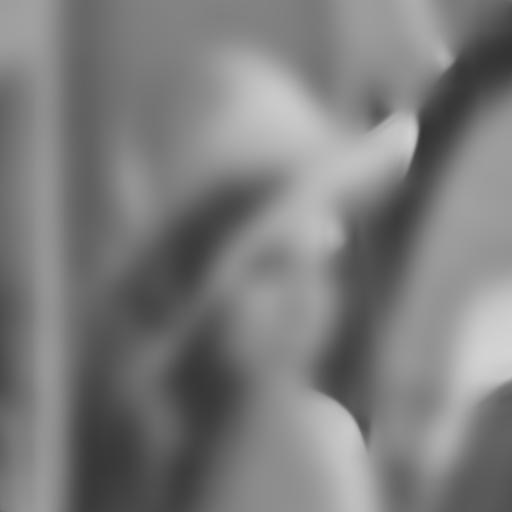
\includegraphics[width=16mm]{Figures/results_wavelet/lena_ric.jpg}}\\
        \subfigure{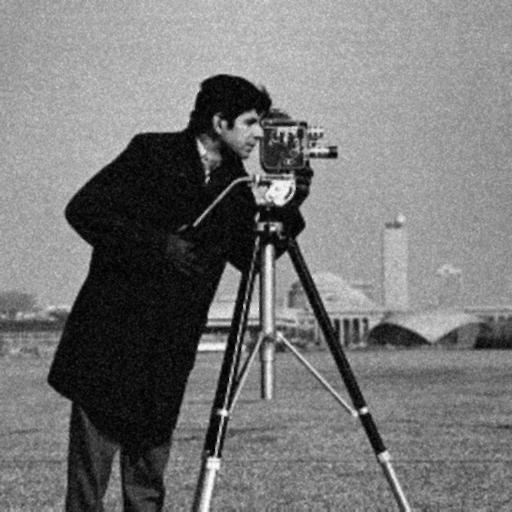
\includegraphics[width=16mm]{Figures/results_wavelet/cameraman_ric.jpg}}\\
        \subfigure{\includegraphics[width=16mm]{Figures/results_wavelet/baboon_ric.jpg}}
      \end{varwidth}
      \begin{varwidth}{0.5\linewidth}
        \subfigure{\includegraphics[width=16mm]{Figures/results_wavelet/lena_uni.jpg}}\\
        \subfigure{\includegraphics[width=16mm]{Figures/results_wavelet/cameraman_uni.jpg}}\\
        \subfigure{\includegraphics[width=16mm]{Figures/results_wavelet/baboon_uni.jpg}}
      \end{varwidth}
      \begin{varwidth}{0.5\linewidth}
        \subfigure{\includegraphics[width=16mm]{Figures/results_wavelet/lena_sp.jpg}}\\
        \subfigure{\includegraphics[width=16mm]{Figures/results_wavelet/cameraman_sp.jpg}}\\
        \subfigure{\includegraphics[width=16mm]{Figures/results_wavelet/baboon_sp.jpg}}
      \end{varwidth}
      \begin{varwidth}{0.5\linewidth}
        \subfigure{\includegraphics[width=16mm]{Figures/results_wavelet/lena_spec.jpg}}\\
        \subfigure{\includegraphics[width=16mm]{Figures/results_wavelet/cameraman_spec.jpg}}\\
        \subfigure{\includegraphics[width=16mm]{Figures/results_wavelet/baboon_spec.jpg}}
      \end{varwidth}
  	\end{tabular}
  \caption{Denoised images with the wavelet filter. From left to right: removing Gaussian, Rician, uniform, salt and pepper and speckle noise, respectively.} 
  \label{fig:results_synthetic_wavelet}
\end{figure}

\begin{figure}[H]
  \centering
 \begin{tabular}{c c c c c}
     \begin{varwidth}{0.5\linewidth}
       \subfigure{\includegraphics[width=16mm]{Figures/results_KSVD/lena_nor.jpg}}\\
       \subfigure{\includegraphics[width=16mm]{Figures/results_KSVD/cameraman_nor.jpg}}\\
       \subfigure{\includegraphics[width=16mm]{Figures/results_KSVD/baboon_nor.jpg}}
     \end{varwidth}
     \begin{varwidth}{0.5\linewidth}
       \subfigure{\includegraphics[width=16mm]{Figures/results_KSVD/lena_ric.jpg}}\\
       \subfigure{\includegraphics[width=16mm]{Figures/results_KSVD/cameraman_ric.jpg}}\\
       \subfigure{\includegraphics[width=16mm]{Figures/results_KSVD/baboon_ric.jpg}}
     \end{varwidth}
     \begin{varwidth}{0.5\linewidth}
       \subfigure{\includegraphics[width=16mm]{Figures/results_KSVD/lena_uni.jpg}}\\
       \subfigure{\includegraphics[width=16mm]{Figures/results_KSVD/cameraman_uni.jpg}}\\
       \subfigure{\includegraphics[width=16mm]{Figures/results_KSVD/baboon_uni.jpg}}
     \end{varwidth}
     \begin{varwidth}{0.5\linewidth}
       \subfigure{\includegraphics[width=16mm]{Figures/results_KSVD/lena_sp.jpg}}\\
       \subfigure{\includegraphics[width=16mm]{Figures/results_KSVD/cameraman_sp.jpg}}\\
       \subfigure{\includegraphics[width=16mm]{Figures/results_KSVD/baboon_sp.jpg}}
     \end{varwidth}
     \begin{varwidth}{0.5\linewidth}
       \subfigure{\includegraphics[width=16mm]{Figures/results_KSVD/lena_spec.jpg}}\\
       \subfigure{\includegraphics[width=16mm]{Figures/results_KSVD/cameraman_spec.jpg}}\\
       \subfigure{\includegraphics[width=16mm]{Figures/results_KSVD/baboon_spec.jpg}}
     \end{varwidth}
 	\end{tabular}
  \caption{Denoised images with the K-SVD filter. From left to right: removing Gaussian, Rician, uniform, salt and pepper and speckle noise, respectively.} 
  \label{fig:results_synthetic_K-SVD}
\end{figure}

In order to easily compare the performance of the different methods, the PSNR results have been grouped according to the different kind of noise that have been analyzed.

\begin{table}[H]
	\centering
	\caption{PSNR for denoising algorithms considering Gaussian noise}
	\begin{tabular}{|c|c|c|c|}
	\hline
	\textbf{Technique} & \textbf{Lena} & \textbf{Cameraman} & \textbf{Baboon} \\ \hline
	Mean & $28.54$ & $28.64$ & $21.77$ \\ \hline
	Median & $27.59$ & $27.88$ & $21.60$ \\ \hline
	LS & $26.53$ & $27.40$ & $\textbf{22.06}$ \\ \hline
	Wavelet & $19.91$ & $20.18$& $17.76$\\ \hline
	K-SVD & $\textbf{28.77}$ & $\textbf{28.86}$ & $21.02$ \\ \hline
	\textbf{Input noise} & $\textbf{20.79}$ & $\textbf{20.37}$ & $\textbf{20.02}$ \\ \hline
	\end{tabular}
	\label{tab:numerical_results_gaussian}
\end{table}

\begin{table}[H]
	\centering
	\caption{PSNR for denoising algorithms considering Rician noise}
	\begin{tabular}{|c|c|c|c|}
	\hline
	\textbf{Technique} & \textbf{Lena} & \textbf{Cameraman} & \textbf{Baboon} \\ \hline
	Mean & $\textbf{29.94}$ & $\textbf{30.29}$ & $22.05$ \\ \hline
	Median & $29.33$ & $29.78$ & $22.04$ \\ \hline
	LS & $27.87$ & $28.82$ & $\textbf{22.46}$ \\ \hline
	Wavelet & $22.61$ & $22.82$ & $19.27$ \\ \hline
	K-SVD & $29.35$  & $29.87$ & $21.50$ \\ \hline
	\textbf{Input noise} & $\textbf{23.20}$ & $\textbf{23.40}$ & $\textbf{23.19}$ \\ \hline
	\end{tabular}
	\label{tab:numerical_results_rician}
\end{table}

\begin{table}[H]
	\centering
	\caption{PSNR for denoising algorithms considering uniform noise}
	\begin{tabular}{|c|c|c|c|}
	\hline
	\textbf{Technique} & \textbf{Lena} & \textbf{Cameraman} & \textbf{Baboon} \\ \hline
	Mean & $28.45$ & $28.57$ & $21.77$ \\ \hline
	Median & $25.99$ & $26.30$ & $21.31$ \\ \hline
	LS & $26.70$ & $27.06$ & $\textbf{22.06}$ \\ \hline
	Wavelet & $19.84$ & $20.16$ & $17.72$\\ \hline
	K-SVD & $\textbf{28.72}$ & $\textbf{28.78}$ & $21.10$ \\ \hline
	\textbf{Input noise} & $\textbf{20.00}$ & $\textbf{20.35}$ & $\textbf{20.00}$ \\ \hline
	\end{tabular}
	\label{tab:numerical_results_uniform}
\end{table}

\begin{table}[H]
	\centering
	\caption{PSNR for denoising algorithms considering salt and pepper noise}
	\begin{tabular}{|c|c|c|c|}
	\hline
	\textbf{Technique} & \textbf{Lena} & \textbf{Cameraman} & \textbf{Baboon} \\ \hline
	Mean & $24.80$ & $24.38$ & $20.72$ \\ \hline
	Median & $\textbf{32.77}$ & $\textbf{33.62}$ & $\textbf{22.22}$\\ \hline
	LS & $23.25$ & $23.14$ & $20.64$ \\ \hline
	Wavelet & $21.18$ & $25.22$ & $15.31$\\ \hline
	K-SVD & $25.47$  & $22.16$ & $19.86$ \\ \hline
	\textbf{Input noise} & $\textbf{15.43}$ & $\textbf{15.11}$ & $\textbf{15.56}$ \\ \hline
	\end{tabular}
	\label{tab:numerical_results_sp}
\end{table}

\begin{table}[H]
	\centering
	\caption{PSNR for denoising algorithms considering speckle noise}
	\begin{tabular}{|c|c|c|c|}
	\hline
	\textbf{Technique} & \textbf{Lena} & \textbf{Cameraman} & \textbf{Baboon} \\ \hline
	Mean & $28.73$ & $22.38$ & $\textbf{28.84}$ \\ \hline
	Median & $27.82$ & $22.11$ & $27.82$ \\ \hline
	LS & $27.47$ & $28.08$ & $20.97$ \\ \hline
	Wavelet & $28.36$ & $28.49$ & $20.97 $\\ \hline
	K-SVD & $\textbf{31.29}$ & $\textbf{30.83}$ & $25.90$ \\ \hline
	\textbf{Input noise} & $\textbf{21.75}$ & $\textbf{21.57}$ & $\textbf{21.76}$ \\ \hline
	\end{tabular}
	\label{tab:numerical_results_speckle}
\end{table}